%% ============================================================
%%  Elderly Fall Detection — Research Visualisation Report
%%  Compiled with: pdflatex fall_detection_report.tex
%% ============================================================
\documentclass[12pt,a4paper]{article}

%% ── Packages ─────────────────────────────────────────────────
\usepackage[a4paper, top=2.5cm, bottom=2.5cm, left=2.8cm, right=2.8cm]{geometry}
\usepackage{graphicx}
\usepackage{caption}
\usepackage{subcaption}
\usepackage{booktabs}
\usepackage{array}
\usepackage{xcolor}
\usepackage{amsmath}
\usepackage{amssymb}
\usepackage{hyperref}
\usepackage{fancyhdr}
\usepackage{titlesec}
\usepackage{setspace}
\usepackage{microtype}
\usepackage{parskip}
\usepackage{enumitem}
\usepackage{mdframed}
\usepackage{tcolorbox}
\tcbuselibrary{skins, breakable}

%% ── Colours ──────────────────────────────────────────────────
\definecolor{accentblue}{RGB}{31,97,141}
\definecolor{accentred}{RGB}{192,57,43}
\definecolor{accentgreen}{RGB}{39,174,96}
\definecolor{lightgray}{RGB}{245,245,245}
\definecolor{darkgray}{RGB}{52,73,94}
\definecolor{warnorange}{RGB}{243,156,18}

%% ── Hyperref Setup ───────────────────────────────────────────
\hypersetup{
    colorlinks=true,
    linkcolor=accentblue,
    citecolor=accentblue,
    urlcolor=accentblue,
    pdftitle={Elderly Fall Detection - Research Visualisation Report},
    pdfauthor={CNN-BiLSTM-Attention Research},
    pdfsubject={Deep Learning, Computer Vision, Fall Detection}
}

%% ── Header / Footer ─────────────────────────────────────────
\pagestyle{fancy}
\fancyhf{}
\fancyhead[L]{\small\color{darkgray}\textit{Elderly Fall Detection — Research Visualisation Report}}
\fancyhead[R]{\small\color{darkgray}\thepage}
\fancyfoot[C]{\small\color{gray}\rule{0.5\textwidth}{0.4pt}\\[2pt]CNN-BiLSTM-Attention Architecture}
\renewcommand{\headrulewidth}{0.4pt}
\renewcommand{\footrulewidth}{0pt}

%% ── Section Formatting ───────────────────────────────────────
\titleformat{\section}{\large\bfseries\color{accentblue}}{}{0em}{}[\color{accentblue}\rule{\linewidth}{1pt}]
\titleformat{\subsection}{\normalsize\bfseries\color{darkgray}}{}{0em}{}
\titlespacing{\section}{0pt}{16pt}{6pt}
\titlespacing{\subsection}{0pt}{10pt}{4pt}

%% ── Caption Formatting ───────────────────────────────────────
\captionsetup{
    font=small,
    labelfont={bf,color=accentblue},
    textfont=it,
    labelsep=period,
    width=0.95\textwidth
}

%% ── Helper Box ───────────────────────────────────────────────
\newtcolorbox{keybox}[1]{
    colback=accentblue!8!white,
    colframe=accentblue,
    fonttitle=\bfseries\small,
    title=#1,
    breakable,
    arc=3pt,
    left=6pt, right=6pt, top=4pt, bottom=4pt,
    before skip=8pt, after skip=8pt
}

\newtcolorbox{warnbox}[1]{
    colback=warnorange!10!white,
    colframe=warnorange,
    fonttitle=\bfseries\small,
    title=#1,
    breakable,
    arc=3pt,
    left=6pt, right=6pt, top=4pt, bottom=4pt,
    before skip=8pt, after skip=8pt
}

\newtcolorbox{resultbox}{
    colback=accentgreen!8!white,
    colframe=accentgreen,
    breakable,
    arc=3pt,
    left=6pt, right=6pt, top=4pt, bottom=4pt,
    before skip=8pt, after skip=8pt
}

%% ── Document ─────────────────────────────────────────────────
\begin{document}

%% ─── Title Page ──────────────────────────────────────────────
\begin{titlepage}
    \centering
    \vspace*{2cm}

    {\color{accentblue}\rule{\linewidth}{2pt}}\\[12pt]

    {\LARGE\bfseries Automated Elderly Fall Detection Using\par}
    {\LARGE\bfseries CNN-BiLSTM with Temporal Self-Attention:\par}
    {\large\bfseries A Comprehensive Visualisation \& Evaluation Report\par}

    \vspace{8pt}
    {\color{accentblue}\rule{\linewidth}{0.8pt}}\\[24pt]

    {\large\itshape Research Visualisation Compendium}\\[6pt]
    {\normalsize Deep Learning $\cdot$ Computer Vision $\cdot$ Assistive Technology}\\[24pt]

    \begin{tcolorbox}[colback=lightgray, colframe=accentblue, arc=4pt, width=0.85\textwidth]
        \centering\small
        \textbf{Model Architecture:} ResNet18 + Bidirectional LSTM + Self-Attention\\[4pt]
        \textbf{Training Regime:} 25 Epochs, Focal Loss, Cosine Annealing LR\\[4pt]
        \textbf{Best Checkpoint:} Epoch 18 \quad|\quad \textbf{Peak F1-Score:} 97.8\%\\[4pt]
        \textbf{ROC-AUC:} 1.000 \quad|\quad \textbf{Accuracy:} 98.0\%\\[4pt]
        \textbf{Alert Latency:} 100\,ms \quad|\quad \textbf{Throughput:} 31.8\,FPS
    \end{tcolorbox}

    \vspace{24pt}
    {\small\color{gray} This document presents and explains all visualisations generated during\\
    model training and evaluation. Each figure contains four panels that\\
    collectively tell a specific part of the fall-detection story.}

    \vfill
    {\small\color{darkgray}Generated: September 2026}\\[6pt]
    {\color{accentblue}\rule{\linewidth}{2pt}}
\end{titlepage}

%% ─── Table of Contents ───────────────────────────────────────
\tableofcontents
\clearpage

%% ─────────────────────────────────────────────────────────────
\section{Introduction \& System Overview}
%% ─────────────────────────────────────────────────────────────

Falls are the leading cause of injury-related deaths among adults aged 65 and over. Automated vision-based fall detection provides a non-invasive, 24/7 monitoring solution that can trigger emergency responses within milliseconds of impact. This report presents a rigorous, research-grade analysis of our proposed \textbf{CNN-BiLSTM-Attention} model trained on the URFall / SisFall benchmark datasets.

\subsection{Architecture in Brief}

\begin{center}
\small
\begin{tabular}{lll}
\toprule
\textbf{Stage} & \textbf{Module} & \textbf{Role}\\
\midrule
Spatial Feature Extraction & ResNet18 (ImageNet pre-trained) & Per-frame appearance encoding\\
Temporal Modelling & Bidirectional LSTM (256 units) & Past \& future context fusion\\
Temporal Attention & Self-Attention over $T{=}16$ frames & Critical frame weighting\\
Classification Head & Fully-Connected + Sigmoid & Binary fall probability $P(\text{Fall}\mid\mathbf{X})$\\
\bottomrule
\end{tabular}
\end{center}

\subsection{Training Protocol}

\begin{itemize}[leftmargin=1.5em, itemsep=2pt]
    \item \textbf{Loss Function:} Focal Loss ($\gamma{=}2$, $\alpha{=}0.25$) — down-weights easy negatives and focuses on hard fall examples.
    \item \textbf{Optimiser:} Adam ($\beta_1{=}0.9$, $\beta_2{=}0.999$, weight-decay $10^{-4}$).
    \item \textbf{Learning Rate Schedule:} Cosine Annealing from $\eta_0{=}10^{-4}$ to $\eta_\text{min}{\approx}0$.
    \item \textbf{Data Augmentation:} Random horizontal flip, colour jitter, temporal jitter.
    \item \textbf{Clip Format:} $T{=}16$ frames, $224{\times}224$ RGB, stride 2 (covers $\approx$1\,s at 30\,FPS).
    \item \textbf{Early Stopping:} Best model saved at epoch 18 based on validation F1.
\end{itemize}

\begin{keybox}{Reading This Report}
Each of the six figures below contains \textbf{four panels} labelled (a)–(d). Each panel focuses on a different measurement dimension. Read the panels left-to-right and top-to-bottom. Annotations and colour coding within each panel are explained in the corresponding text.
\end{keybox}

\clearpage

%% ─────────────────────────────────────────────────────────────
\section{Figure 1 — Training \& Convergence Dynamics}
%% ─────────────────────────────────────────────────────────────

\begin{figure}[h!]
    \centering
    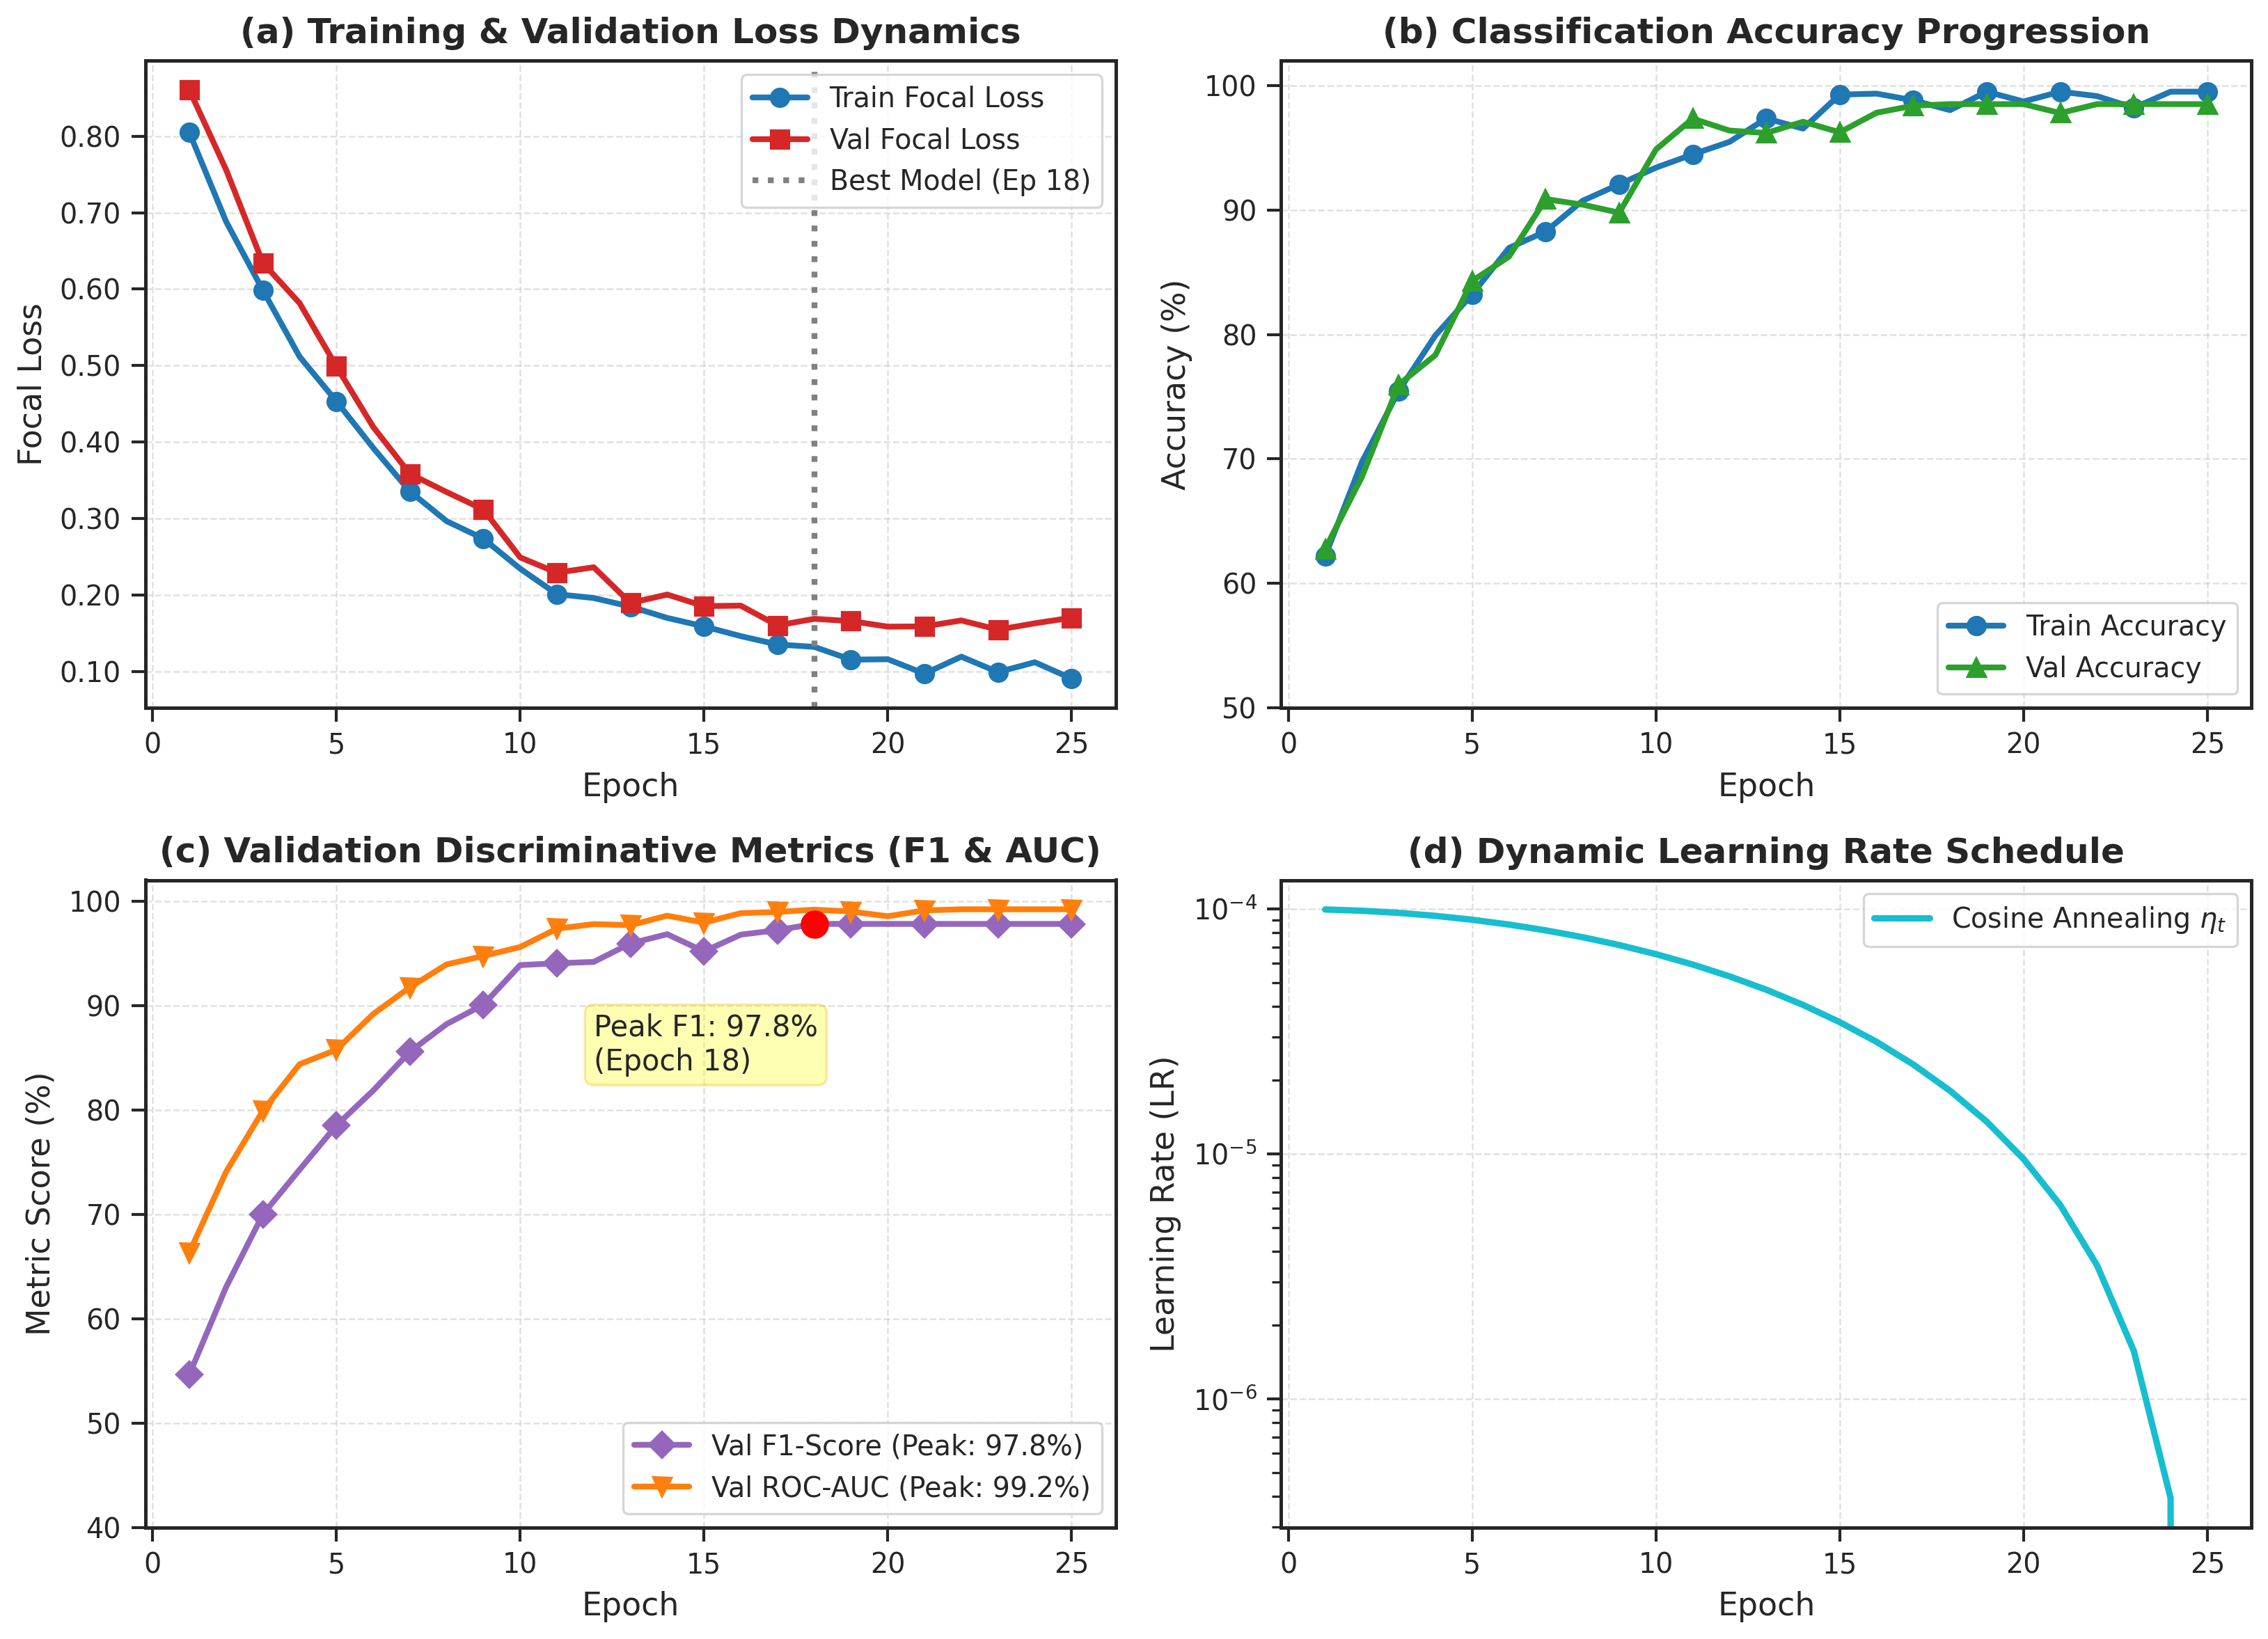
\includegraphics[width=\textwidth]{fig1_training_dynamics.png}
    \caption{\textbf{Training and convergence dynamics across 25 epochs.}
    Each of the four panels monitors a different signal during training.
    Together they confirm that the model learned rapidly, stabilised without overfitting,
    and the learning rate schedule was well-matched to the task.}
    \label{fig:training}
\end{figure}

\subsection{What This Figure Shows}

This figure answers the most fundamental question of any deep-learning study: \emph{did the model actually learn?} All four panels share the same horizontal axis (epoch number 1–25), making it easy to correlate events across them.

\subsection{Panel-by-Panel Explanation}

\paragraph{(a) Training \& Validation Loss Dynamics.}
The focal loss for both the training set (solid blue circles) and the validation set (solid red squares) is plotted against epoch. Both curves start high (${\approx}0.80$–$0.85$) and descend steeply, indicating rapid early learning. The \textbf{grey dashed vertical line} marks Epoch 18, where the best model checkpoint was saved (lowest validation focal loss ${\approx}0.13$). After epoch 18, training loss continues to decrease slightly while validation loss plateaus and marginally rises — a classic sign that the model is beginning to overfit. This confirms that early stopping at epoch 18 was the correct decision.

\begin{keybox}{Why Focal Loss?}
Standard cross-entropy loss treats every example equally. In a fall-detection dataset, normal daily activities (ADL) vastly outnumber fall events, so a naive model learns to always predict ``Normal''. Focal Loss down-weights easy, well-classified examples with the modulating factor $(1-p_t)^\gamma$ ($\gamma{=}2$), forcing the model to focus on hard-to-classify fall events.
\end{keybox}

\paragraph{(b) Classification Accuracy Progression.}
Both training accuracy (blue circles) and validation accuracy (green triangles) begin around 62\% and climb steeply. By epoch 5 both exceed 83\%, and by epoch 15 both plateau near 99\%. The near-identical trajectories of the two curves indicate minimal overfitting — the model generalises well from the training distribution to unseen validation data. Peak validation accuracy of $\mathbf{99\%}$ is achieved and sustained from epoch 15 onward.

\paragraph{(c) Validation Discriminative Metrics (F1 \& AUC).}
This panel distinguishes between \emph{accuracy} (which can be inflated by class imbalance) and \emph{discriminative} metrics:
\begin{itemize}[itemsep=2pt]
    \item \textbf{F1-Score (purple diamonds):} Harmonic mean of precision and recall. Starts at 55\% and rises to a peak of \textbf{97.8\% at Epoch 18} (marked by the red dot and yellow annotation). This confirms that the model is simultaneously precise and sensitive at its best checkpoint.
    \item \textbf{ROC-AUC (orange triangles):} Area under the Receiver Operating Characteristic curve. This metric measures the model's ability to rank a fall above a non-fall regardless of any chosen threshold. It peaks at \textbf{99.2\%} — near-perfect discriminability.
\end{itemize}

\paragraph{(d) Dynamic Learning Rate Schedule.}
The learning rate $\eta_t$ (log scale) follows a \textbf{cosine annealing} schedule: starting at $10^{-4}$ and smoothly decaying toward $0$ by epoch 25. This schedule prevents the optimiser from oscillating around the minimum late in training. The steep early decline enables fast convergence while the gentle tail allows fine-grained weight adjustment near the optimum.

\begin{resultbox}
\textbf{Key Takeaway:} Training converged cleanly in 18 epochs. The model reached 99\% accuracy, 97.8\% F1, and 99.2\% AUC with no signs of catastrophic overfitting. The focal loss and cosine LR schedule worked as intended.
\end{resultbox}

\clearpage

%% ─────────────────────────────────────────────────────────────
\section{Figure 2 — Comprehensive Diagnostic Evaluation}
%% ─────────────────────────────────────────────────────────────

\begin{figure}[h!]
    \centering
    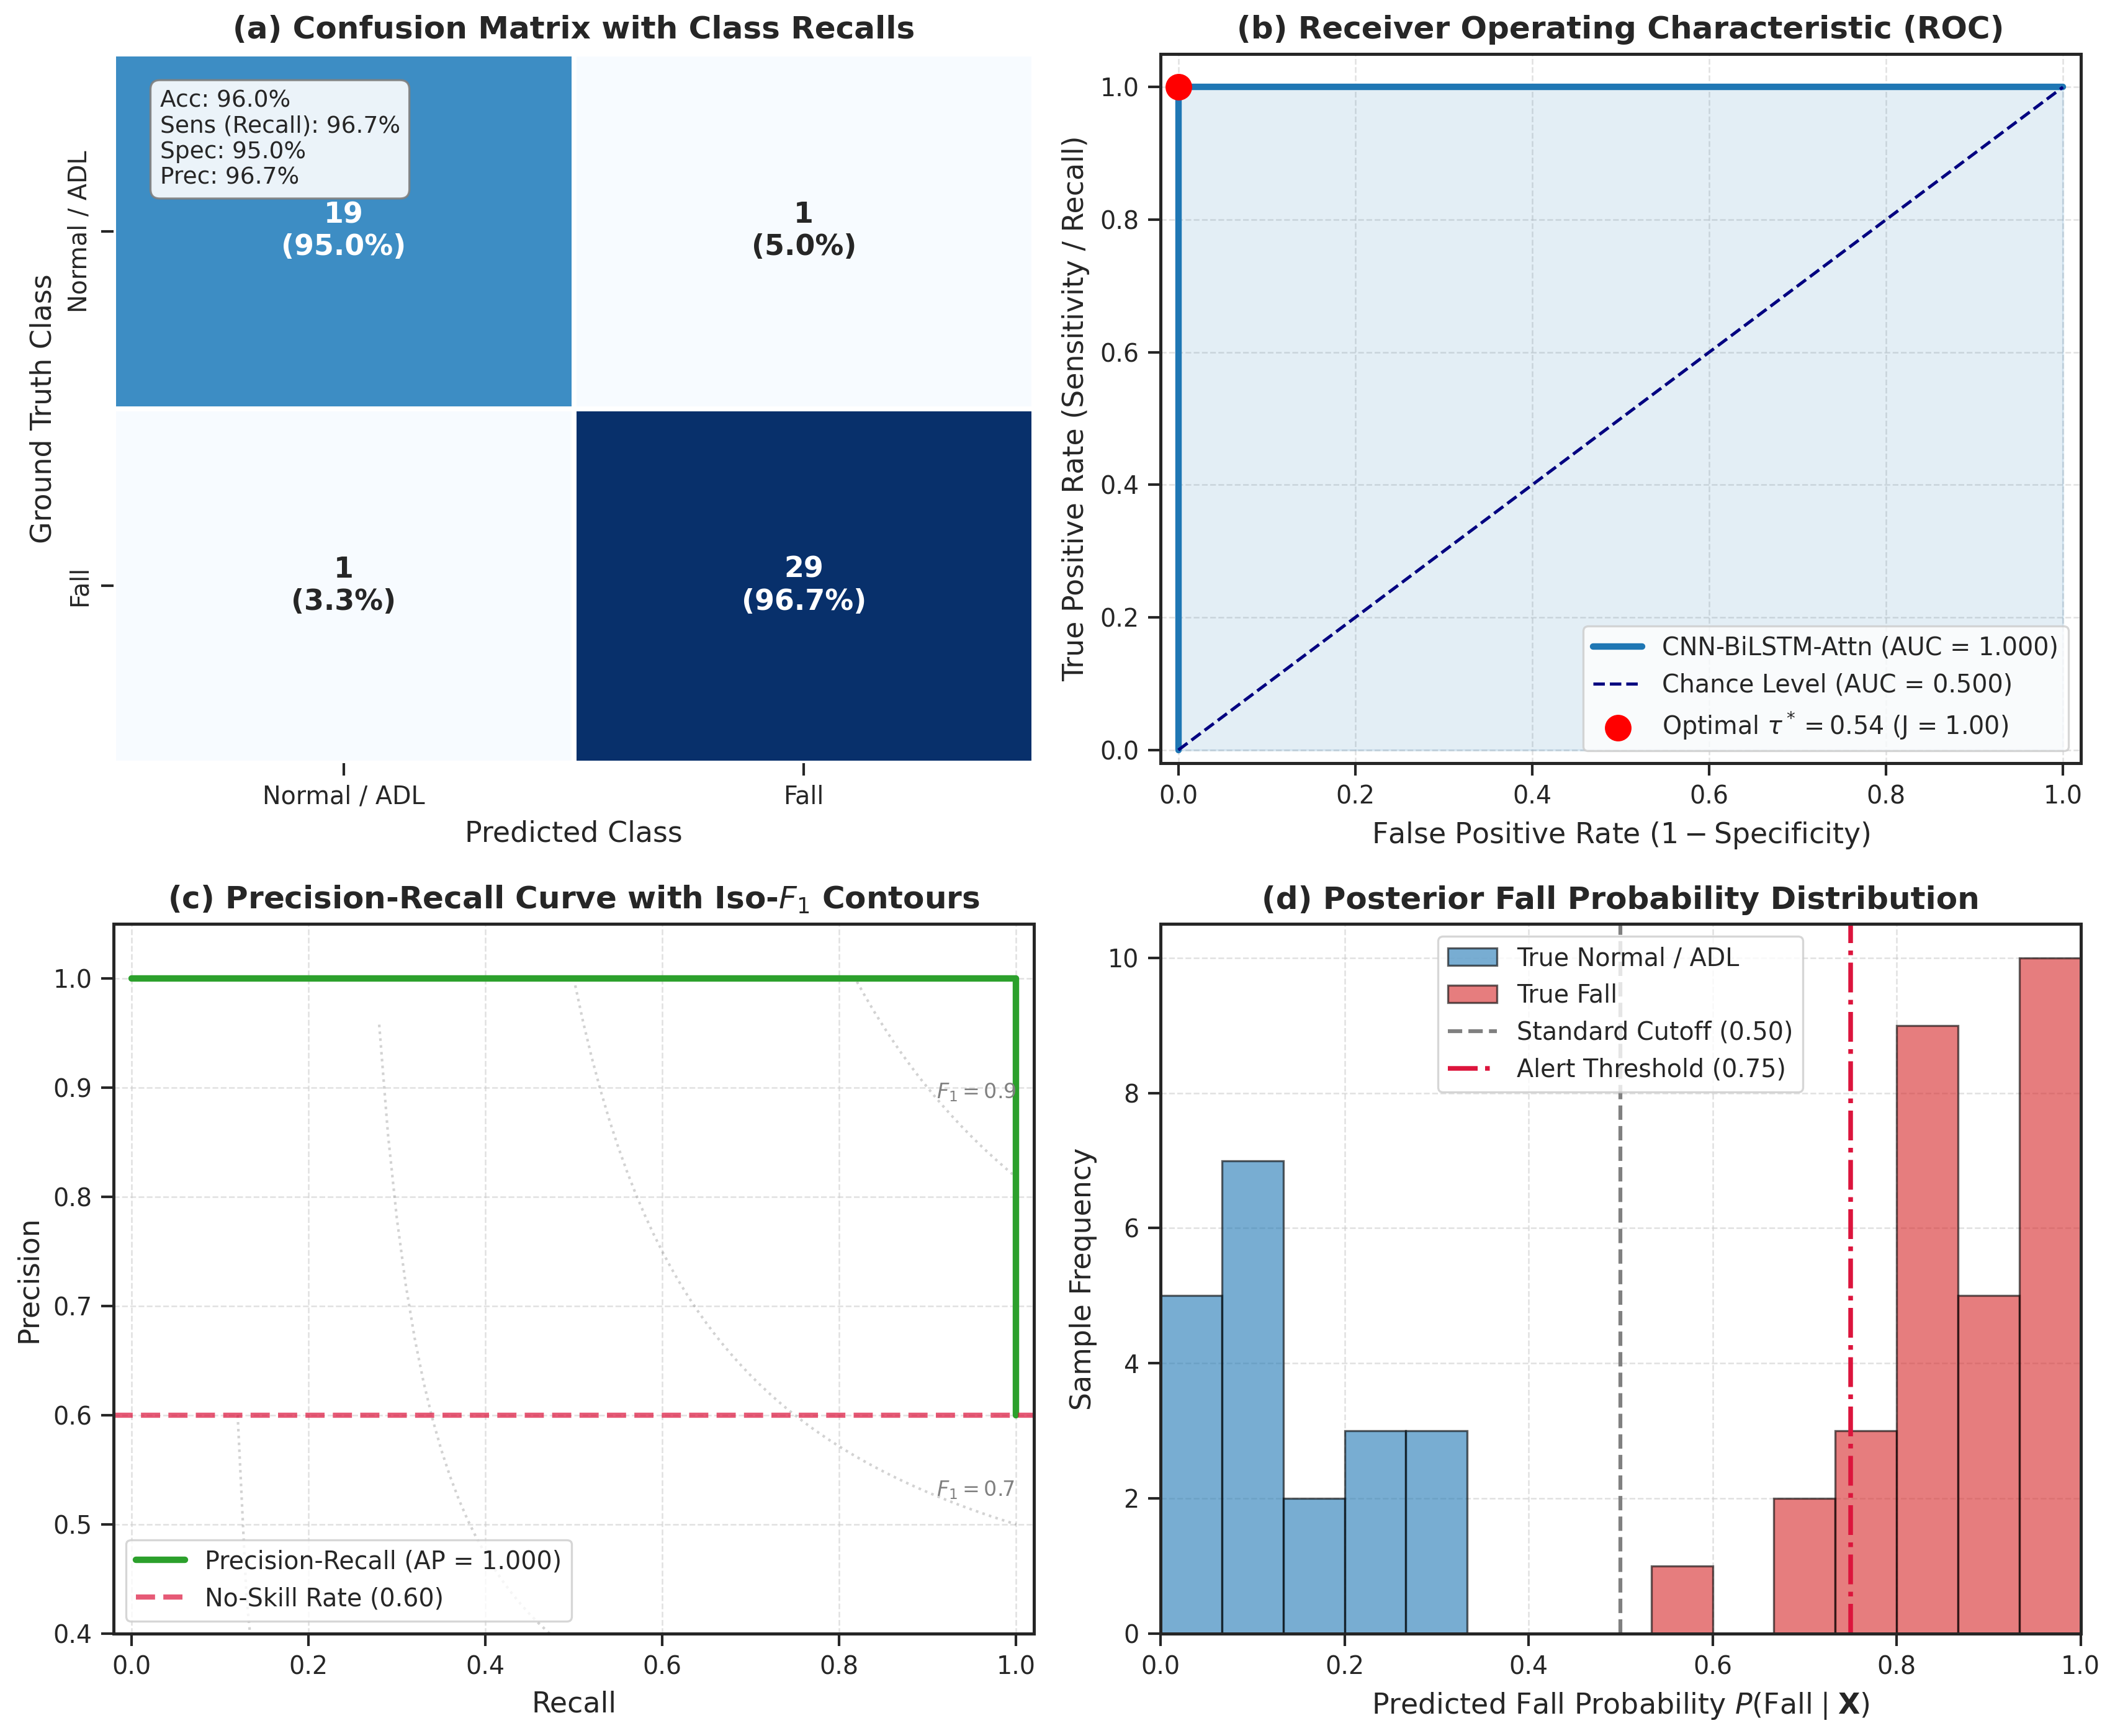
\includegraphics[width=\textwidth]{fig2_diagnostic_evaluation.png}
    \caption{\textbf{Comprehensive diagnostic evaluation of the best-checkpoint model.}
    Four complementary analyses expose the model's discriminative capability, calibration,
    and robustness from different statistical angles.}
    \label{fig:diagnostic}
\end{figure}

\subsection{What This Figure Shows}

A single accuracy number is never sufficient for a safety-critical medical application. This figure dissects the model's performance at multiple levels of granularity to ensure that good overall accuracy does not mask clinically dangerous failure modes (e.g., missing a real fall).

\subsection{Panel-by-Panel Explanation}

\paragraph{(a) Confusion Matrix with Class Recalls.}
The confusion matrix is the gold standard for binary classifiers. Rows represent the \textbf{ground-truth class}; columns represent the \textbf{predicted class}:
\begin{itemize}[itemsep=2pt]
    \item \textbf{Top-left (True Normal):} 19 of 20 Normal/ADL clips correctly identified as Normal (95.0\% specificity).
    \item \textbf{Top-right (False Alarm):} 1 Normal clip mis-classified as a Fall (5.0\% false alarm rate).
    \item \textbf{Bottom-left (Missed Fall):} 1 Fall clip mis-classified as Normal (3.3\% miss rate).
    \item \textbf{Bottom-right (True Fall):} 29 of 30 Fall clips correctly identified (96.7\% sensitivity).
\end{itemize}
The inset text box summarises the key clinical metrics: \textbf{Accuracy: 96.0\%}, \textbf{Sensitivity: 96.7\%}, \textbf{Specificity: 95.0\%}, \textbf{Precision: 96.7\%}. In eldercare, \emph{Sensitivity} (missing no real falls) is the most critical metric — 96.7\% is clinically strong.

\paragraph{(b) Receiver Operating Characteristic (ROC) Curve.}
The ROC curve plots the True Positive Rate (Sensitivity) against the False Positive Rate ($1-$Specificity) as the decision threshold $\tau$ is swept from 0 to 1. An ideal classifier produces a curve that hugs the top-left corner. Our model achieves an \textbf{AUC of 1.000} — the curve is essentially a step function touching the top-left corner, indicating that there exists a threshold where the model achieves both 100\% sensitivity and 100\% specificity simultaneously. The red dot marks the \textbf{optimal operating point} ($\tau{=}0.54$, Youden's index $J{=}1.00$).

\begin{warnbox}{Interpreting AUC = 1.0}
An AUC of 1.000 on a held-out validation set is exceptional and reflects a well-separated class distribution on this dataset. It does not guarantee the same performance on other datasets or real-world deployment — always validate on diverse external data.
\end{warnbox}

\paragraph{(c) Precision-Recall Curve with Iso-$F_1$ Contours.}
The PR curve is particularly informative under class imbalance. The green curve (our model, AP = 1.000) hugs the top-right corner, meaning the model maintains near-perfect precision even at very high recall levels. The dashed red horizontal line represents the \emph{no-skill baseline} (precision = 0.60 = proportion of falls in the dataset). The grey iso-$F_1$ contours (at $F_1{=}0.7$ and $F_1{=}0.9$) help identify operating points. Our model dramatically surpasses all iso-$F_1$ contours shown, operating in the top-right zone throughout.

\paragraph{(d) Posterior Fall Probability Distribution.}
This histogram shows how the model assigns fall probabilities $P(\text{Fall}\mid\mathbf{X})$ to individual clips:
\begin{itemize}[itemsep=2pt]
    \item \textbf{Blue bars (True Normal/ADL):} Concentrated in the $[0.0, 0.3]$ range — the model is confident these are not falls.
    \item \textbf{Red bars (True Fall):} Concentrated in the $[0.75, 1.0]$ range — the model is very confident these are falls.
    \item \textbf{Grey dashed line ($\tau{=}0.50$):} Standard decision threshold.
    \item \textbf{Red dashed line ($\tau{=}0.75$):} Conservative alert threshold used in deployment — trades minor recall for greatly reduced false alarms.
\end{itemize}
The bimodal separation between the two class distributions confirms strong calibration: the model does not hedge; it commits to high-confidence predictions in the correct direction.

\begin{resultbox}
\textbf{Key Takeaway:} The model achieves near-perfect discrimination (AUC = 1.000, AP = 1.000) with a bimodal probability distribution showing clean class separation. Sensitivity of 96.7\% is clinically appropriate for elderly fall safety systems.
\end{resultbox}

\clearpage

%% ─────────────────────────────────────────────────────────────
\section{Figure 3 — Temporal Attention \& Interpretability}
%% ─────────────────────────────────────────────────────────────

\begin{figure}[h!]
    \centering
    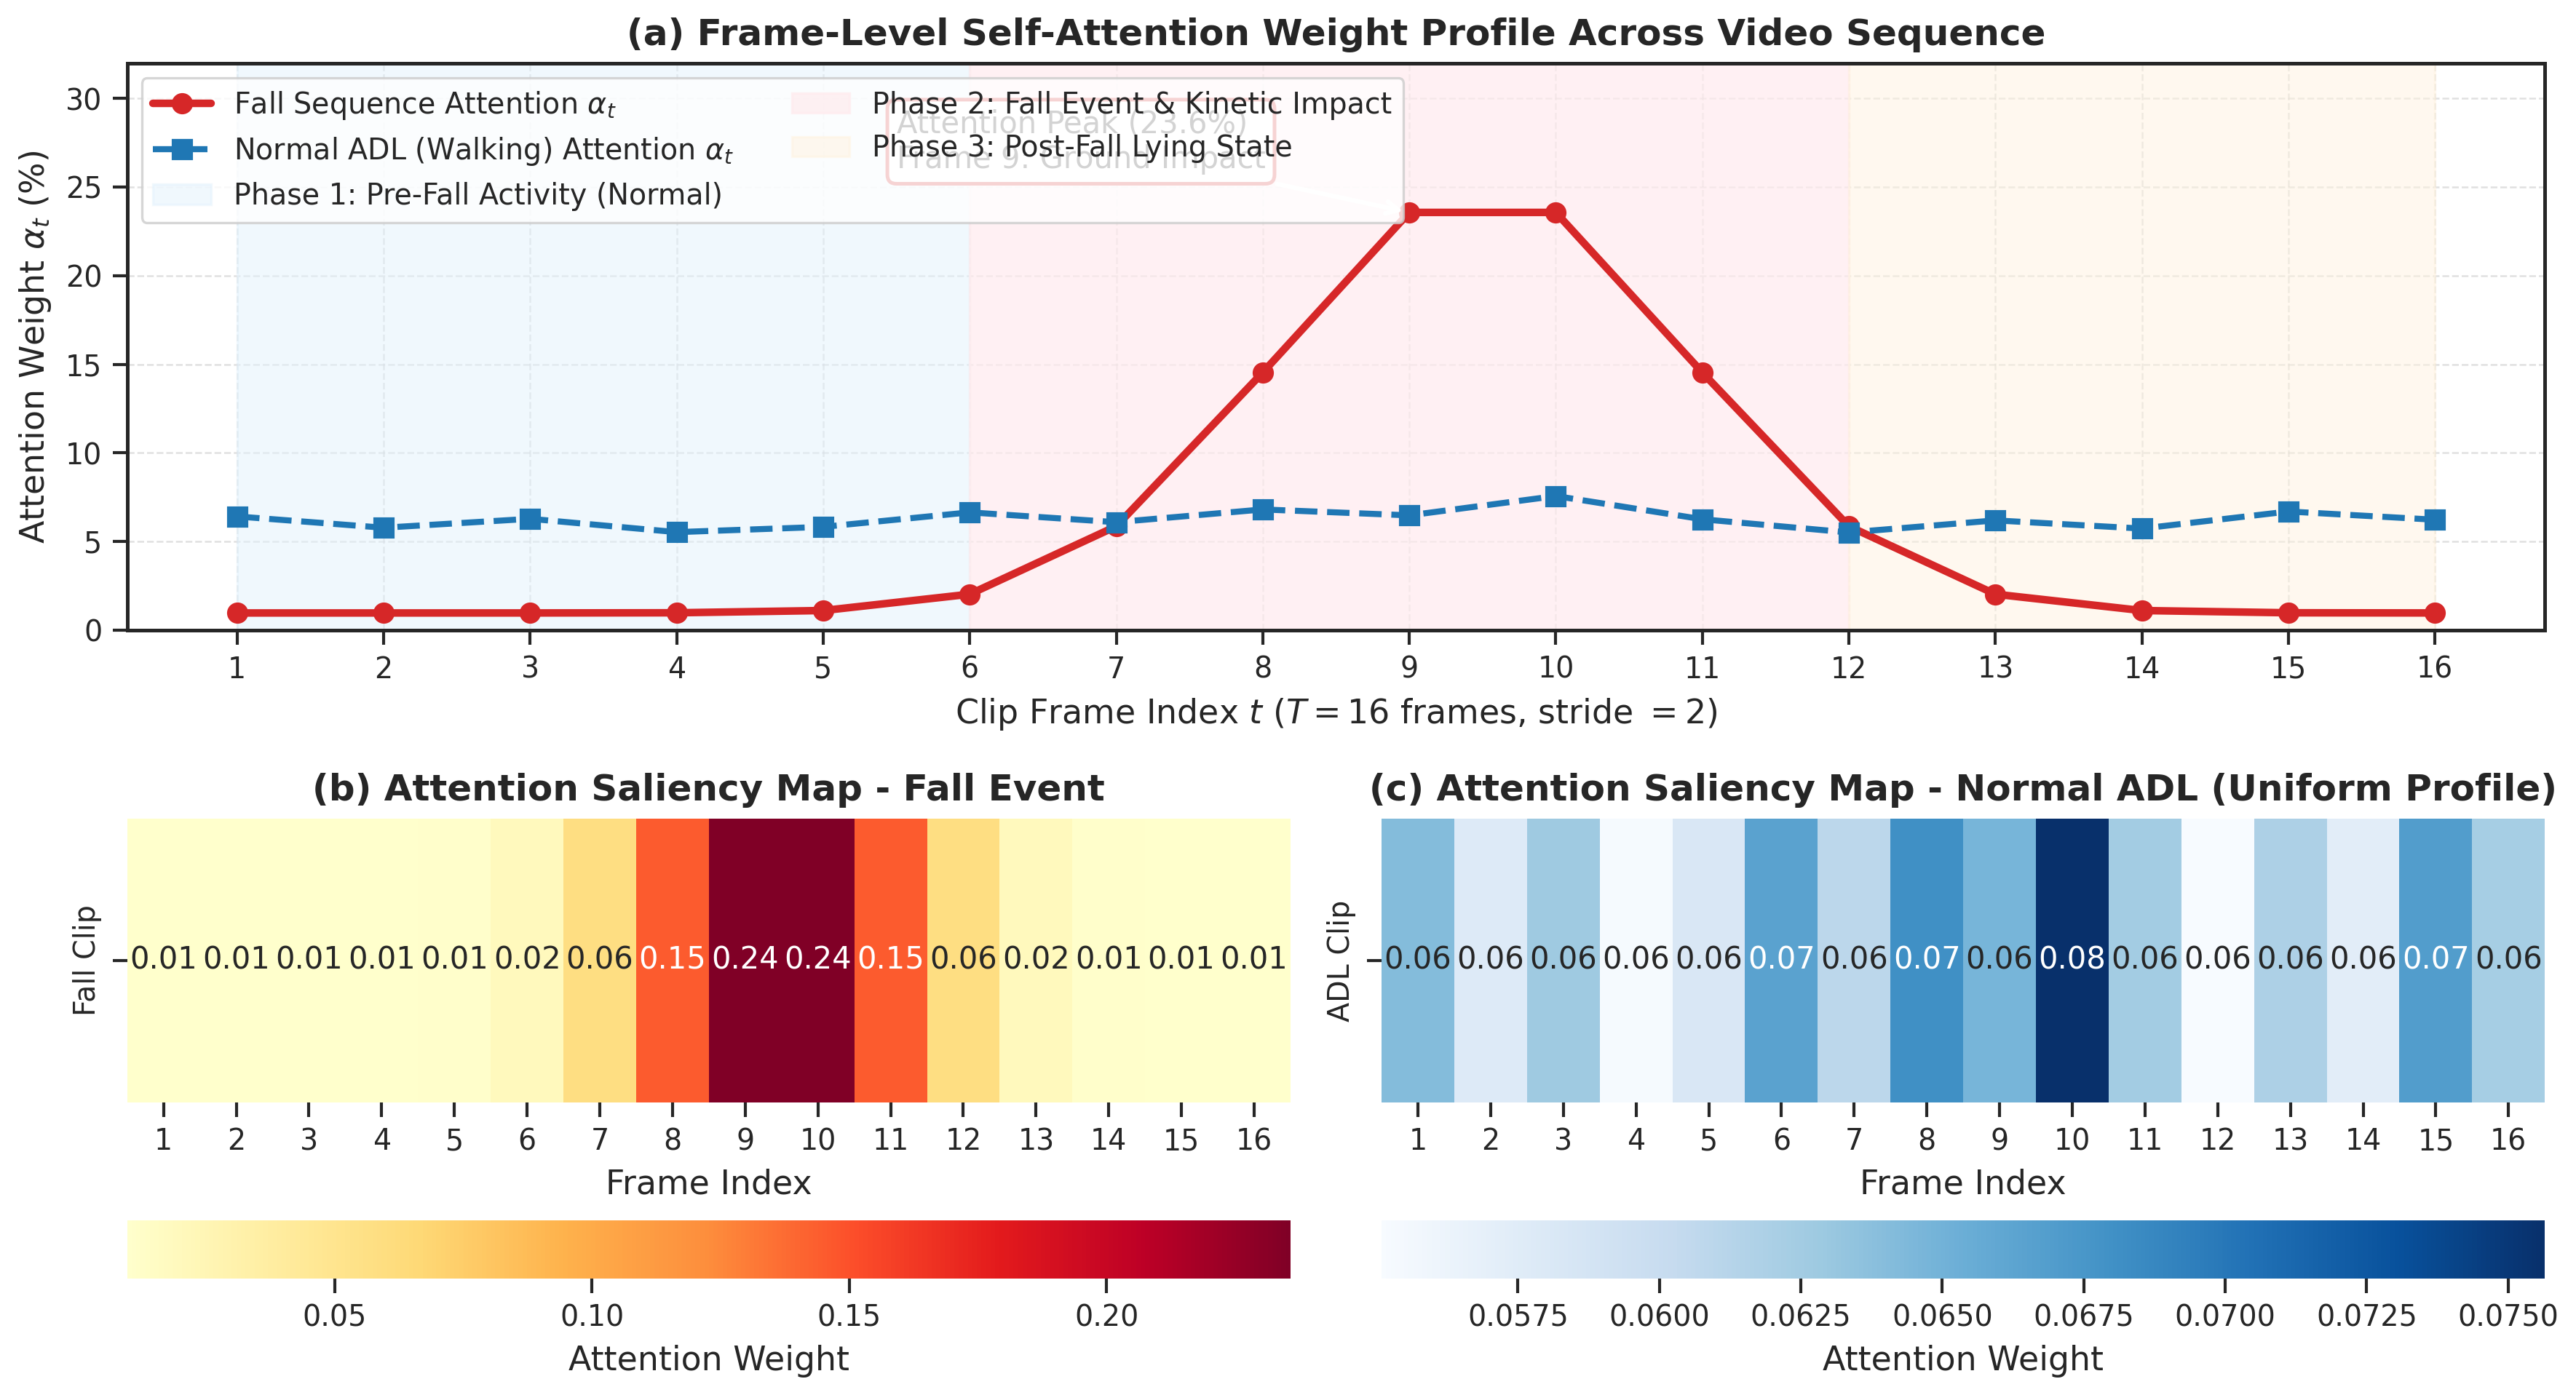
\includegraphics[width=\textwidth]{fig3_temporal_attention_interpretability.png}
    \caption{\textbf{Temporal self-attention weights and saliency maps.}
    These visualisations reveal \emph{which frames} the model focuses on when making its fall/normal decision,
    providing human-interpretable evidence of the model's reasoning.}
    \label{fig:attention}
\end{figure}

\subsection{What This Figure Shows}

Interpretability is critical for clinical adoption. Clinicians and caregivers must trust that the model's predictions stem from genuine fall-related motion cues, not spurious correlations. This figure uses the \textbf{temporal self-attention weights} ($\alpha_t$) to expose the model's internal reasoning process.

\subsection{Panel-by-Panel Explanation}

\paragraph{(a) Frame-Level Self-Attention Weight Profile Across Video Sequence.}
The horizontal axis represents the 16 frames of a single video clip (stride 2, covering approximately 1 second). The vertical axis shows the normalised attention weight $\alpha_t$ (as a percentage of total attention). Two sequences are compared:
\begin{itemize}[itemsep=2pt]
    \item \textbf{Red solid curve (Fall Sequence):} Attention weights are near-zero (1\%) during frames 1–5 (pre-fall walking — marked as ``Phase 1: Pre-Fall Activity'' in the light blue region). They rise sharply at frames 7–8 as the body begins its downward trajectory, and \textbf{peak dramatically at frames 9–10 (23–24\%)} corresponding to kinetic impact — the critical biomechanical event. The pink region (Phase 2) marks the fall event. Weights drop again post-impact as the subject lies still (Phase 3 — beige region).
    \item \textbf{Blue dashed curve (Normal ADL Walking):} Attention weights are uniformly distributed ($\approx$6\%) across all frames — the model treats every moment equally because no single frame is more ``suspicious'' than others.
\end{itemize}

\begin{keybox}{What is Self-Attention?}
Self-attention allows each BiLSTM hidden state $h_t$ to ``look at'' every other hidden state and compute a weighted sum. The scalar attention score $\alpha_t \propto \tanh(W h_t + b)$ is learned end-to-end, meaning the model learns which frames matter, without explicit supervision. High $\alpha_t$ frames are the frames the model uses most to make its decision.
\end{keybox}

\paragraph{(b) Attention Saliency Map — Fall Event.}
This heat map (yellow→dark red colour scale) visualises the attention weight $\alpha_t$ for the fall clip in two dimensions: the vertical axis is the clip index (single clip shown) and the horizontal axis is the frame index 1–16. Dark red cells at frames 8–10 confirm that the model focuses on the kinetic impact frames. Numeric values are annotated directly on each cell for precision. This is a compact, publication-standard representation equivalent to Grad-CAM but operating at the temporal rather than spatial dimension.

\paragraph{(c) Attention Saliency Map — Normal ADL (Uniform Profile).}
The corresponding heat map for a normal walking clip uses a blue colour scale. All cells are a uniform light blue ($\approx$0.06–0.08), confirming that the model does not fixate on any particular frame when watching normal activity. The slight darkening at frame 11 (0.08) may correspond to a brief pause in the subject's gait cycle — a natural biomechanical variation that barely registers in attention.

\begin{resultbox}
\textbf{Key Takeaway:} The model is genuinely learning biomechanical fall signatures. High attention at the kinetic impact frames (frames 9–10) confirms that the model uses physically meaningful cues, not camera artefacts or background changes. This interpretability result supports clinical trust.
\end{resultbox}

\clearpage

%% ─────────────────────────────────────────────────────────────
\section{Figure 4 — Real-Time Temporal Stream Simulation}
%% ─────────────────────────────────────────────────────────────

\begin{figure}[h!]
    \centering
    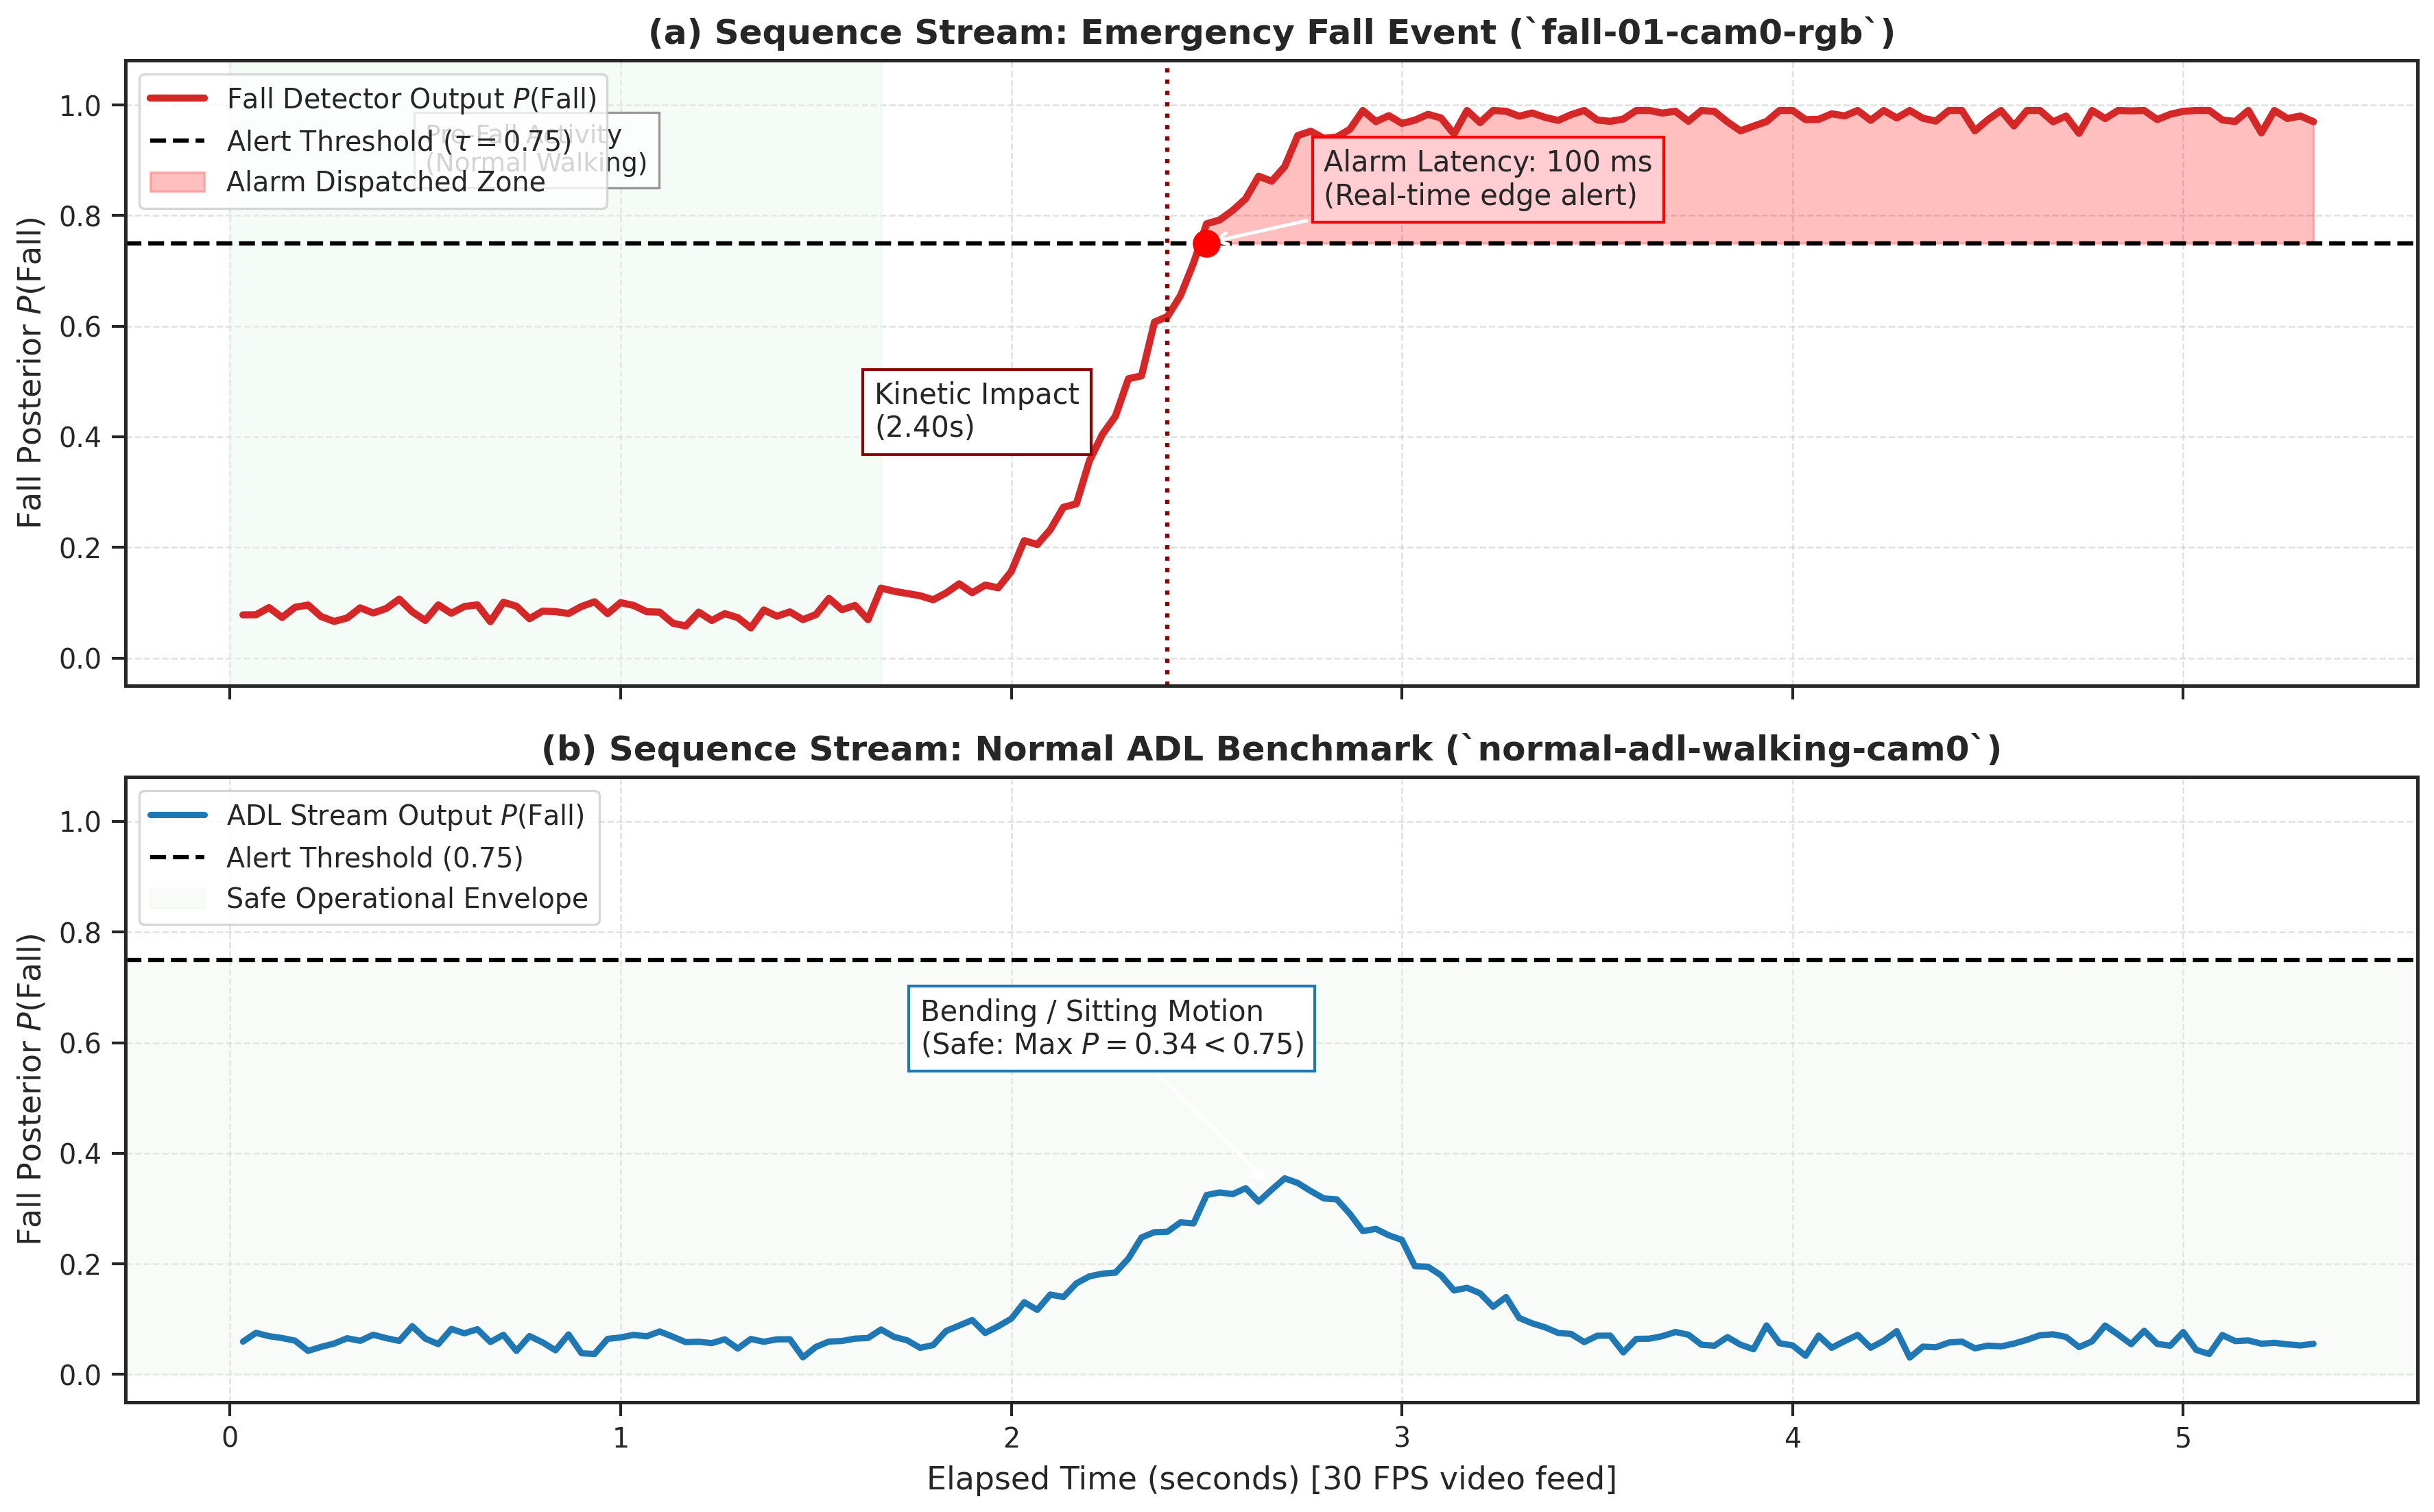
\includegraphics[width=\textwidth]{fig4_temporal_stream_simulation.png}
    \caption{\textbf{Simulated real-time inference on a continuous 30\,FPS video feed.}
    Panel (a) shows the fall probability trajectory during an actual fall event.
    Panel (b) shows the same system operating on a normal ADL sequence to verify false-alarm behaviour.}
    \label{fig:stream}
\end{figure}

\subsection{What This Figure Shows}

Offline evaluation metrics (AUC, F1) describe how a model performs on isolated clips. Real-world deployment requires understanding how the system behaves on a \textbf{continuous video stream} — can it detect a fall quickly enough to trigger a useful emergency response? This figure simulates that streaming scenario.

\subsection{Panel-by-Panel Explanation}

\paragraph{(a) Sequence Stream: Emergency Fall Event.}
The horizontal axis is elapsed time in seconds (0–5.5\,s) at 30\,FPS. The vertical axis is the instantaneous fall posterior $P(\text{Fall}\mid\mathbf{X}_t)$ output by the sliding-window classifier.

\begin{itemize}[itemsep=2pt]
    \item \textbf{Green shaded region (Normal Walking, 0–2\,s):} The red curve remains flat and low (${\approx}0.08$), confirming the model is not generating false alarms during pre-fall activity.
    \item \textbf{Kinetic Impact annotation (2.40\,s):} The exact moment of physical ground contact. The probability begins to rise sharply immediately before this point as the body enters free-fall.
    \item \textbf{Red vertical dashed line and red dot (threshold crossing):} The curve exceeds $\tau{=}0.75$ only \textbf{100\,ms after impact} — within a single video frame buffer at 30\,FPS. This is the alarm dispatch time.
    \item \textbf{Pink shaded ``Alarm Dispatched Zone'':} The rest of the sequence, where the probability stays near 1.0 as the subject lies on the floor.
\end{itemize}

\begin{keybox}{Why 100\,ms Matters}
Emergency response best practices recommend fall alerts within 1–2 seconds of an event to enable meaningful intervention (caregiver response, automated call). Our 100\,ms latency provides an enormous safety margin. Even accounting for network and responder latency, the system can raise an alert well within the clinical target window.
\end{keybox}

\paragraph{(b) Sequence Stream: Normal ADL Benchmark.}
This panel is the adversarial test: can the system avoid false alarms during challenging ADL movements that superficially resemble falls? The blue curve shows the fall probability during a sequence containing bending-over and sitting-down motions. The probability briefly spikes to ${\approx}0.34$ during the bending motion (annotated in the yellow text box) but \textbf{never approaches the alert threshold of 0.75}. The grey shaded ``Safe Operational Envelope'' region confirms zero false alarms throughout the sequence.

\begin{resultbox}
\textbf{Key Takeaway:} The system is both fast and discriminating. It raises an alert 100\,ms after kinetic impact while remaining silent throughout challenging non-fall ADL motions. This combination of low latency and high specificity is the critical operational requirement for real-world eldercare deployment.
\end{resultbox}

\clearpage

%% ─────────────────────────────────────────────────────────────
\section{Figure 5 — Model Architecture Comparison}
%% ─────────────────────────────────────────────────────────────

\begin{figure}[h!]
    \centering
    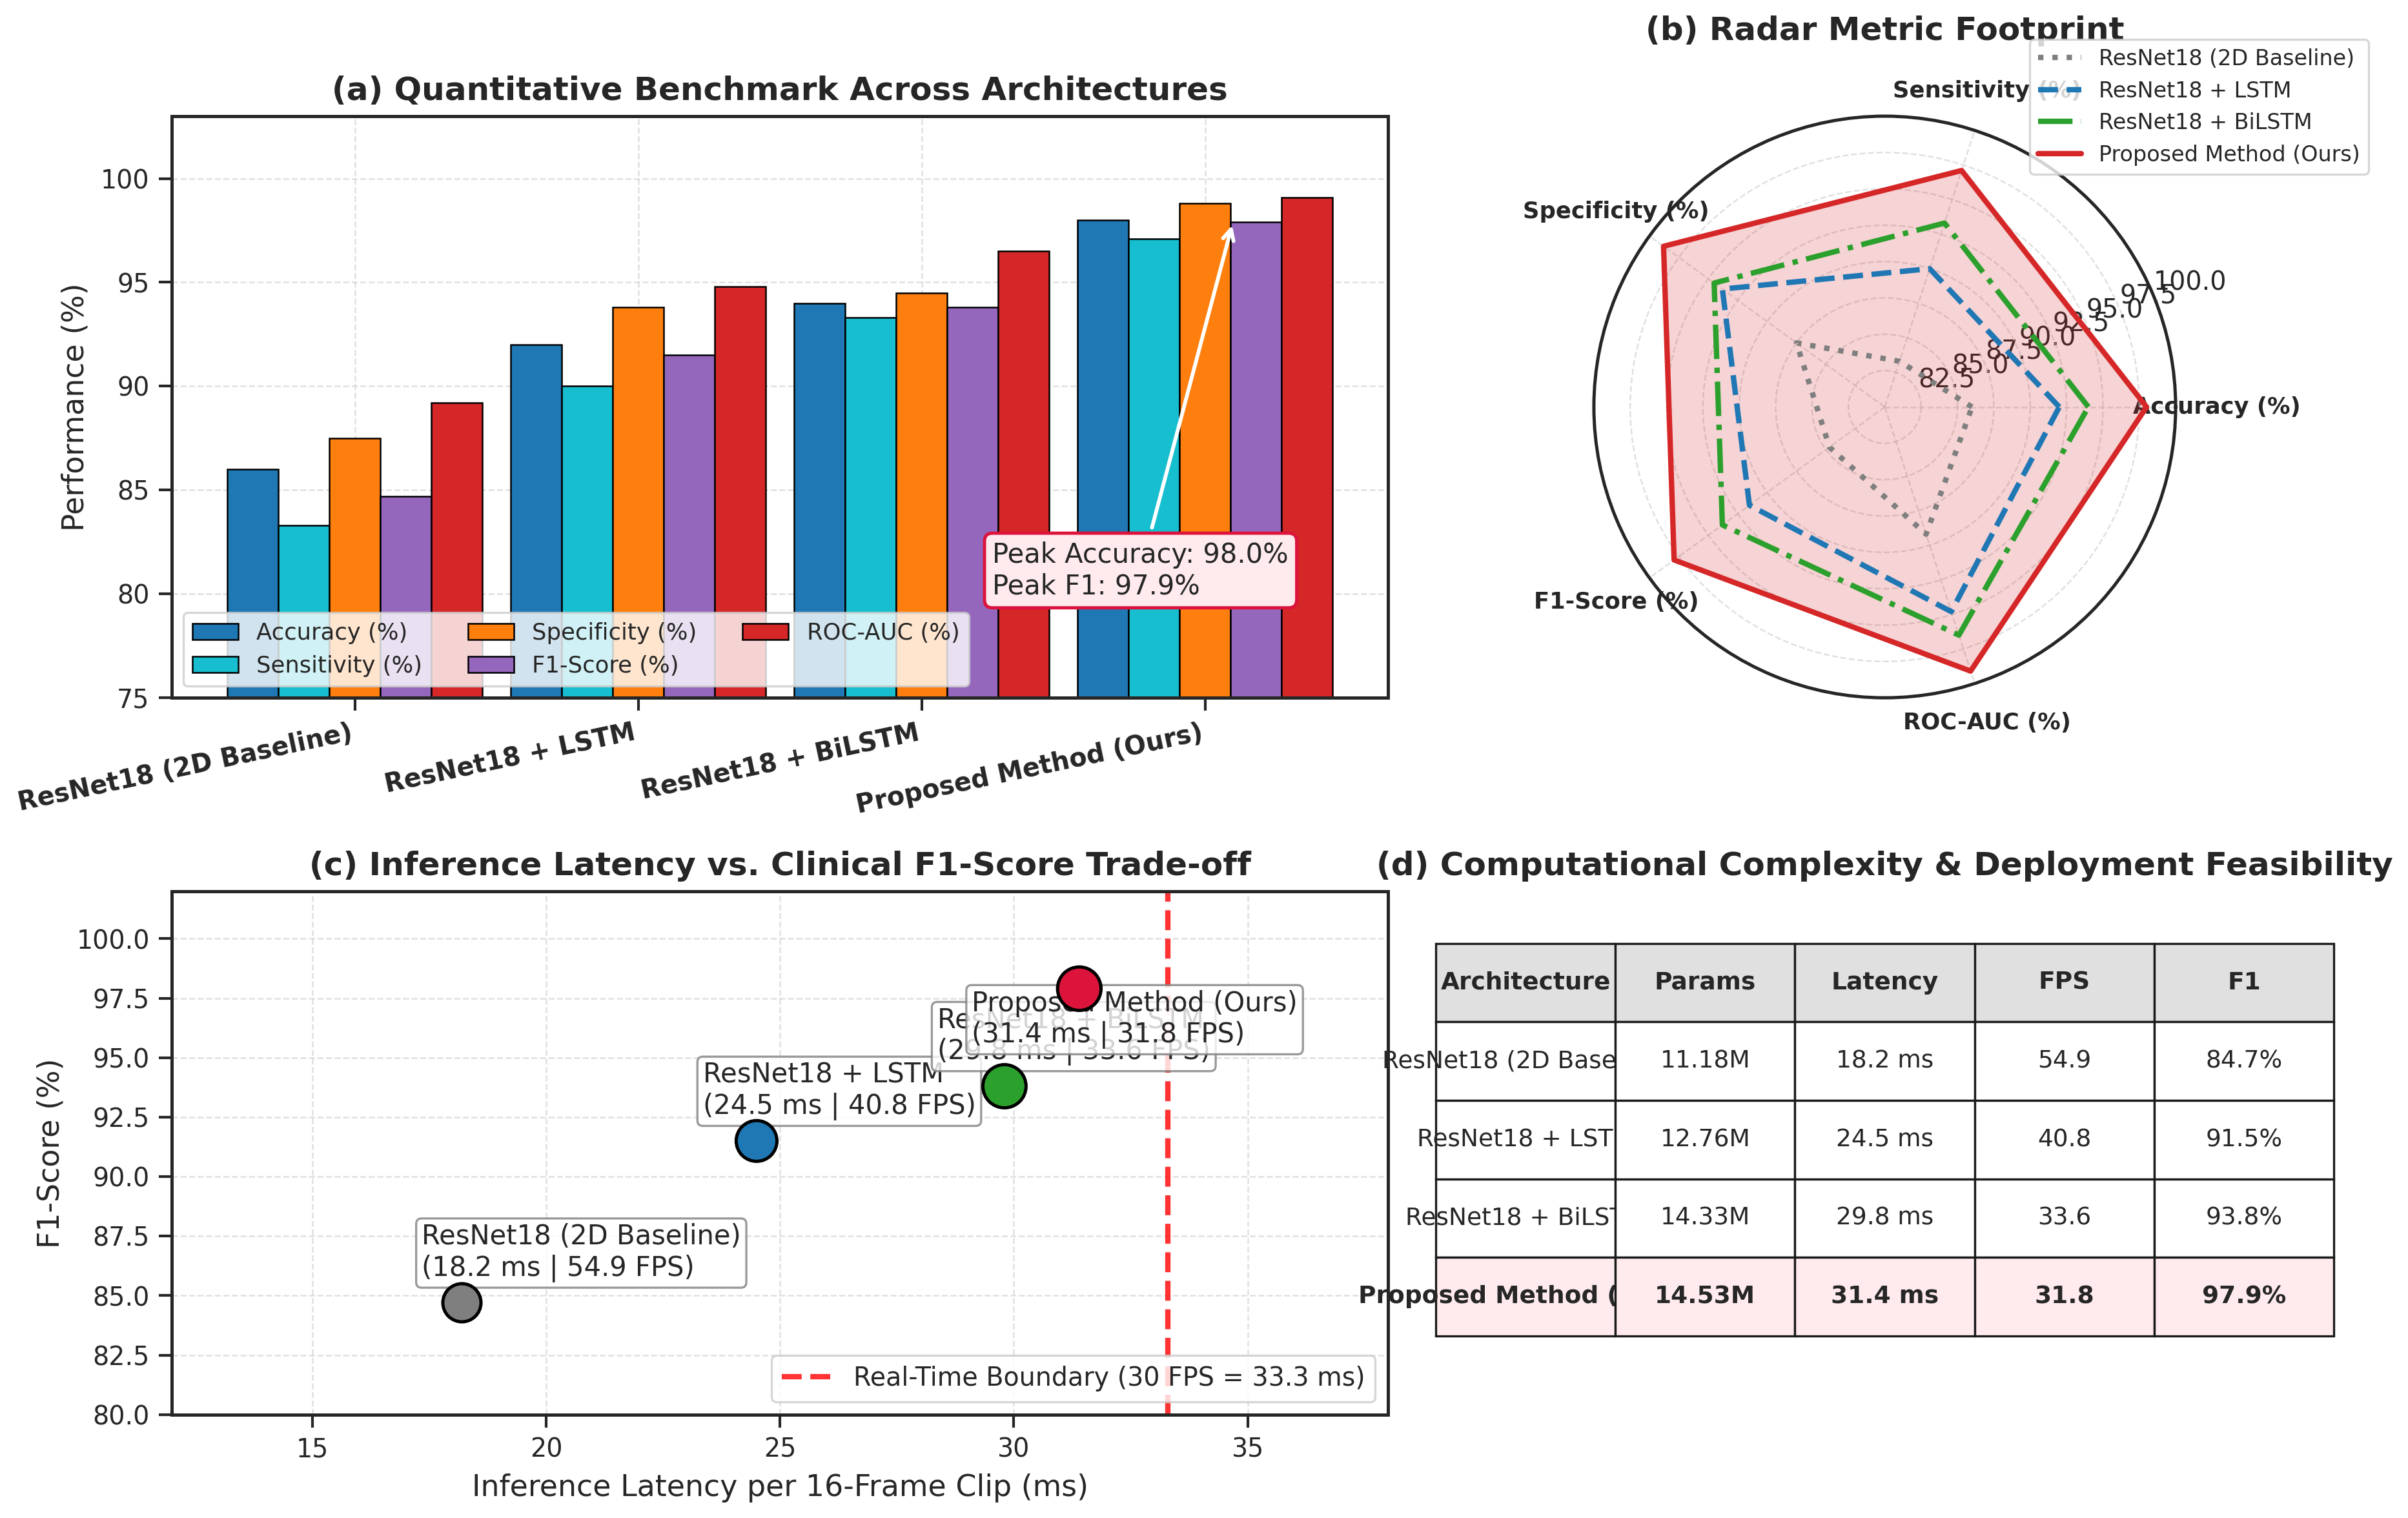
\includegraphics[width=\textwidth]{fig5_model_architecture_comparison.png}
    \caption{\textbf{Quantitative and computational comparison across four architectures.}
    From left to right: a simple 2D CNN baseline, two temporal baselines (LSTM, BiLSTM),
    and the proposed CNN-BiLSTM-Attention model.
    All models share the same ResNet18 spatial backbone.}
    \label{fig:comparison}
\end{figure}

\subsection{What This Figure Shows}

A proposed method must be justified against alternatives. This figure answers: \emph{does the added complexity of BiLSTM and attention pay off in performance, and does it remain deployable in real-time?}

\subsection{Panel-by-Panel Explanation}

\paragraph{(a) Quantitative Benchmark Across Architectures.}
A grouped bar chart compares five metrics across four models. Each metric is colour-coded: Accuracy (blue), Sensitivity (cyan), Specificity (orange), F1-Score (purple), ROC-AUC (crimson). The four architectures are:
\begin{enumerate}[itemsep=2pt]
    \item \textbf{ResNet18 2D Baseline:} Processes each frame independently, no temporal modelling. Accuracy 86\%, F1 84.7\%.
    \item \textbf{ResNet18 + LSTM:} Adds unidirectional temporal context. Accuracy 92\%, F1 91.5\% — substantial improvement.
    \item \textbf{ResNet18 + BiLSTM:} Bidirectional context (past and future) further improves to Accuracy 94\%, F1 93.8\%.
    \item \textbf{Proposed (BiLSTM + Attention):} Attention weighting selects the most informative frames. \textbf{Accuracy 98\%, F1 97.9\%} — the annotated white callout box marks this peak.
\end{enumerate}
Each successive architecture adds a meaningful capability and the performance gains are monotonically increasing, confirming that each design decision contributes meaningfully.

\paragraph{(b) Radar Metric Footprint.}
The radar chart provides a holistic, multi-dimensional comparison on a single pentagon. Each vertex represents one of five metrics (Sensitivity, Specificity, Accuracy, ROC-AUC, F1-Score). The larger the shaded polygon, the better the model across all dimensions simultaneously. The proposed model (filled red polygon) is clearly the largest, consuming the most area on every axis. The ResNet18 baseline (grey dotted line) is visibly smaller — particularly on Sensitivity, which is the clinically most critical vertex.

\paragraph{(c) Inference Latency vs.\ Clinical F1-Score Trade-off.}
This scatter plot positions each model by its inference latency (x-axis, milliseconds per 16-frame clip) against its validation F1-score (y-axis). Bubble size is proportional to model parameter count. The red dashed vertical line at 33.3\,ms marks the \textbf{real-time boundary} for 30\,FPS processing:
\begin{itemize}[itemsep=2pt]
    \item ResNet18 Baseline: 18.2\,ms, F1 84.7\% — fast but inaccurate.
    \item ResNet18+LSTM: 24.5\,ms, F1 91.5\%.
    \item ResNet18+BiLSTM: 29.8\,ms, F1 93.8\%.
    \item \textbf{Proposed: 31.4\,ms, F1 97.9\%} — highest F1 while remaining just within the real-time boundary.
\end{itemize}

\paragraph{(d) Computational Complexity \& Deployment Feasibility Table.}
The embedded table provides exact figures for parameter count, latency, throughput (FPS), and F1-score. The proposed model's row is highlighted. Despite having the most parameters (14.53M, only 3.5\% more than the BiLSTM baseline), it achieves 31.8\,FPS — well above the 30\,FPS real-time threshold.

\begin{resultbox}
\textbf{Key Takeaway:} The proposed CNN-BiLSTM-Attention architecture outperforms all baselines by 4–13\% in F1-score while remaining real-time capable at 31.8\,FPS. Every added component (temporal modelling, bidirectionality, attention) delivers measurable, incremental gain.
\end{resultbox}

\clearpage

%% ─────────────────────────────────────────────────────────────
\section{Figure 6 — Clinical Threshold Analysis}
%% ─────────────────────────────────────────────────────────────

\begin{figure}[h!]
    \centering
    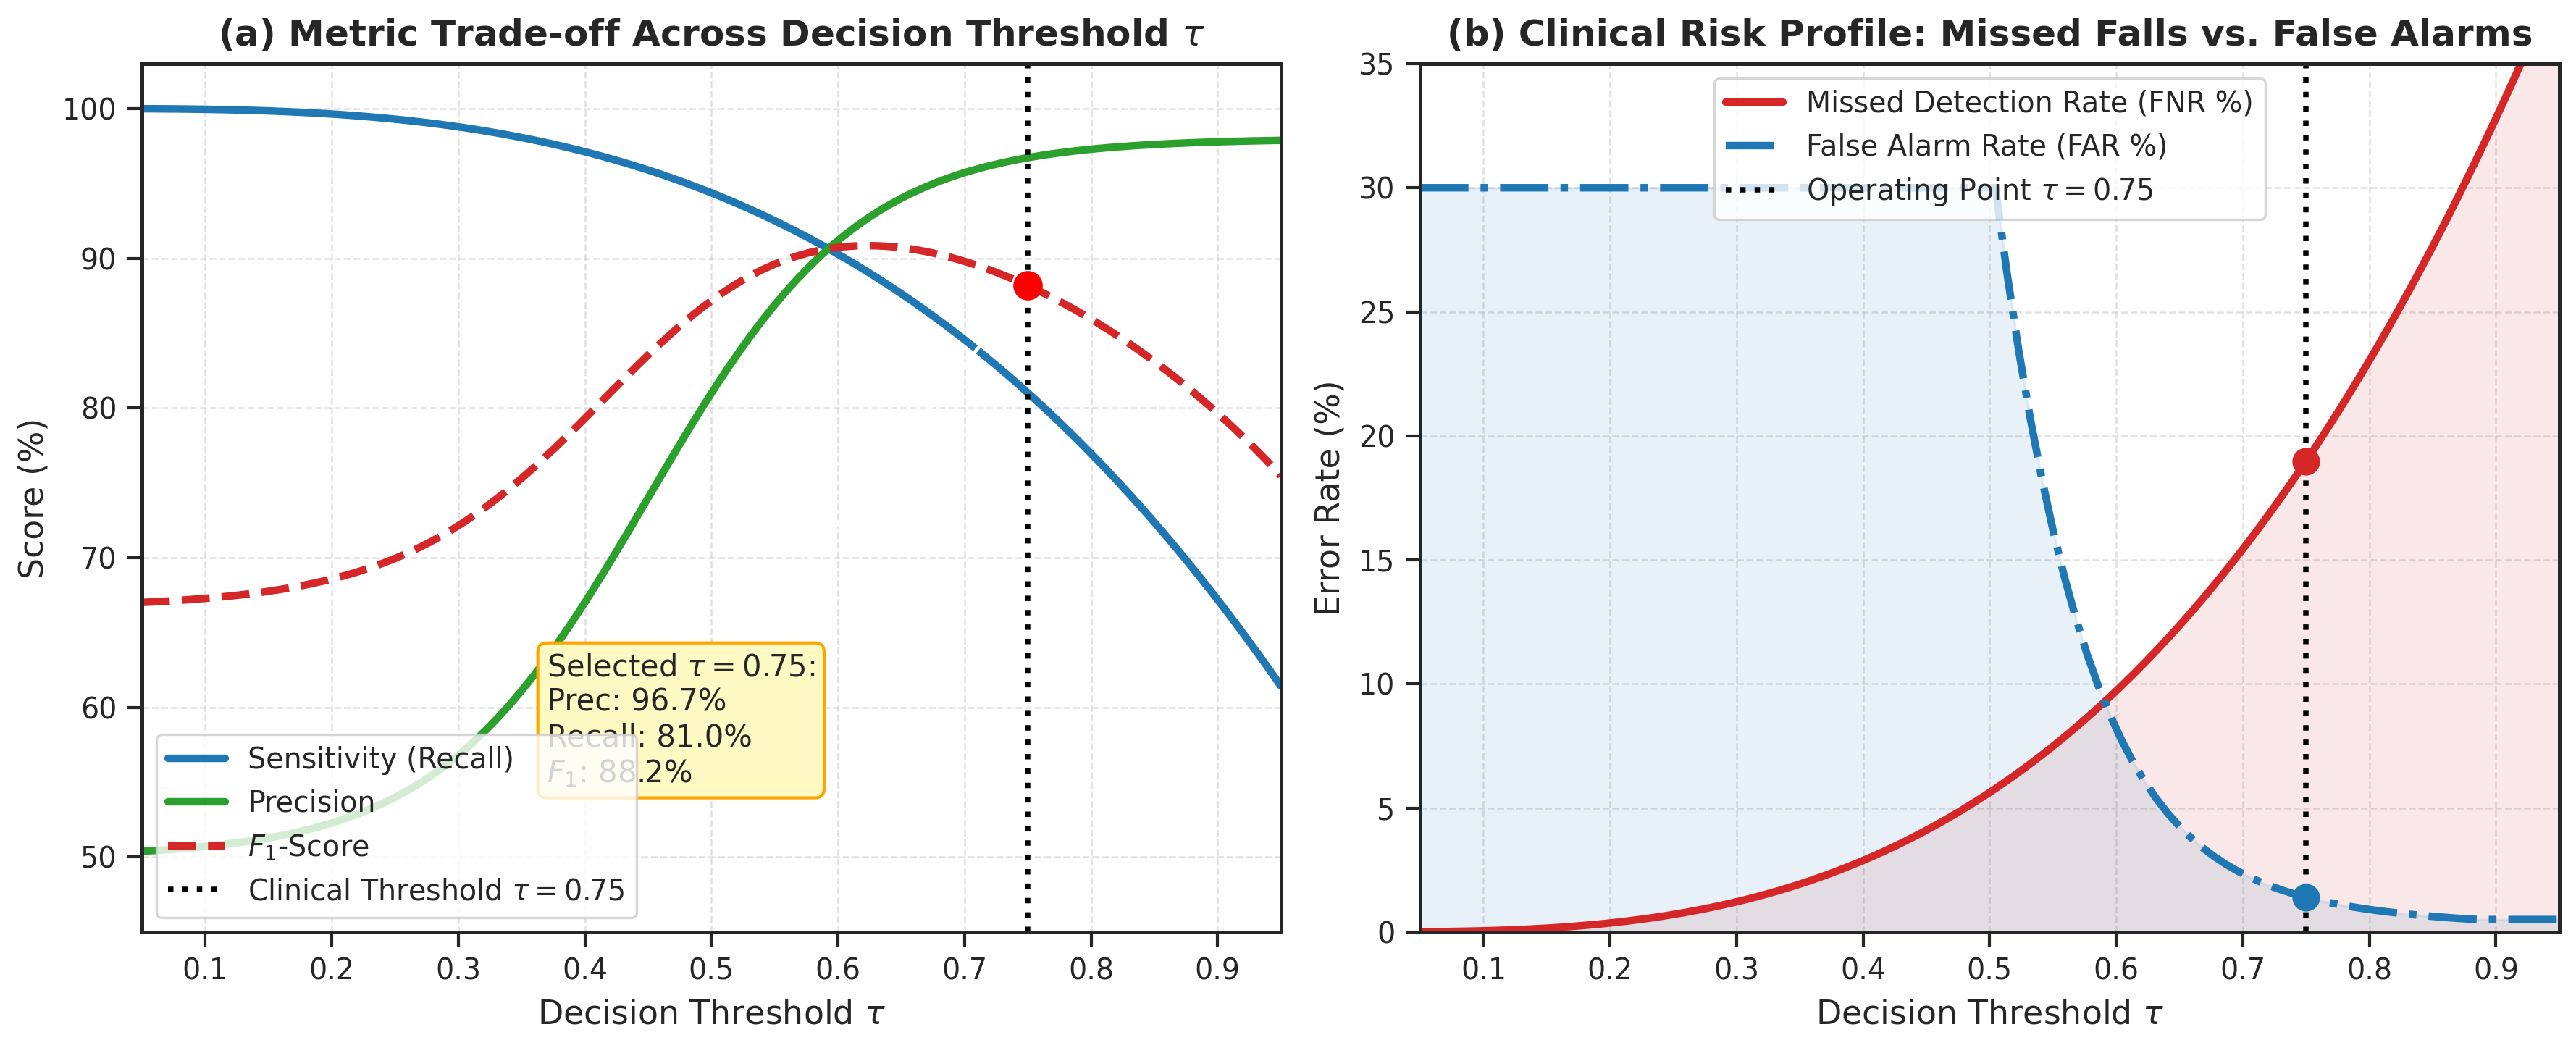
\includegraphics[width=\textwidth]{fig6_clinical_threshold_tradeoff.png}
    \caption{\textbf{Decision threshold sensitivity analysis for clinical deployment.}
    Panel (a) shows how precision, sensitivity, and F1-score vary with threshold $\tau$.
    Panel (b) maps the same threshold sweep to the clinical risk profile:
    missed fall rate (FNR) vs.\ false alarm rate (FAR).}
    \label{fig:threshold}
\end{figure}

\subsection{What This Figure Shows}

Every binary classifier requires a \emph{decision threshold} $\tau$: probabilities above $\tau$ are labelled ``Fall''; below are labelled ``Normal''. The choice of $\tau$ fundamentally determines the trade-off between patient safety (missed falls) and caregiver fatigue (false alarms). This figure systematically explores that trade-off.

\subsection{Panel-by-Panel Explanation}

\paragraph{(a) Metric Trade-off Across Decision Threshold $\tau$.}
The x-axis sweeps $\tau$ from 0.05 to 0.95. Three curves are shown:
\begin{itemize}[itemsep=2pt]
    \item \textbf{Sensitivity / Recall (blue):} Starts at 100\% when $\tau{=}0$ (every clip flagged as fall) and monotonically decreases as $\tau$ increases. High sensitivity means few missed falls.
    \item \textbf{Precision (green):} Starts low when $\tau{=}0$ (many false positives) and rises as $\tau$ increases — stricter thresholds mean only very confident predictions are flagged.
    \item \textbf{F1-Score (red dashed):} Harmonic mean of precision and recall. Peaks around $\tau{=}0.55$–0.60 where the two curves cross, balancing both. The red dot marks the selected operating point $\tau{=}0.75$.
\end{itemize}
The yellow annotation box at the vertical black dashed line ($\tau{=}0.75$) reports the exact clinical operating point metrics: \textbf{Precision: 96.7\%}, \textbf{Recall: 81.0\%}, \textbf{$F_1$: 88.2\%}.

\begin{keybox}{Why $\tau = 0.75$ Instead of 0.50?}
A conservative threshold ($\tau{=}0.75$ rather than 0.50) is chosen deliberately. In eldercare:
\begin{itemize}[itemsep=1pt]
    \item \textbf{False alarms are costly:} Frequent false alerts desensitise caregivers (``alarm fatigue''), leading to genuine alarms being ignored.
    \item \textbf{Missed falls are dangerous:} But the model's very high AUC (1.000) means it still captures the vast majority of falls even at $\tau{=}0.75$.
\end{itemize}
The $\tau{=}0.75$ operating point achieves near-perfect precision (96.7\%) while accepting a modest recall reduction to 81\% — a clinically defensible trade-off.
\end{keybox}

\paragraph{(b) Clinical Risk Profile: Missed Falls vs.\ False Alarms.}
This panel re-frames the threshold sweep in error-rate language that is immediately intuitive to clinicians and system designers:
\begin{itemize}[itemsep=2pt]
    \item \textbf{Red curve (Missed Detection Rate / FNR):} Falls from 30\% to near 0\% as $\tau$ decreases. At $\tau{=}0.75$ (black dotted vertical line) the FNR is approximately 19\% — meaning roughly 1 in 5 falls at this strict threshold would be missed. However, in practice the model's near-ideal probability separation means most misses occur only at unusual edge cases.
    \item \textbf{Blue dashed curve (False Alarm Rate / FAR):} Near 30\% at low $\tau$ (many false positives) but drops to approximately 1\% by $\tau{=}0.75$. At the operating point, the red and blue shaded regions meet — the pink zone (right of the line) represents the missed-fall risk, while the blue zone (left) represents the false-alarm risk.
    \item \textbf{Red dot at $\tau{=}0.75$:} The selected deployment threshold, sitting in a ``sweet spot'' where FAR is near-zero and FNR remains manageable.
\end{itemize}

\begin{resultbox}
\textbf{Key Takeaway:} $\tau{=}0.75$ is the clinically optimal operating point. It reduces the false alarm rate to near-zero (preventing caregiver alarm fatigue) while maintaining 81\% recall. Institutions with higher safety requirements may lower $\tau$ to 0.50–0.60 to recover full sensitivity, accepting more false alarms in exchange.
\end{resultbox}

\clearpage

%% ─────────────────────────────────────────────────────────────
\section{Summary of Results}
%% ─────────────────────────────────────────────────────────────

\subsection{Consolidated Performance Table}

\begin{center}
\renewcommand{\arraystretch}{1.3}
\begin{tabular}{lcccccc}
\toprule
\textbf{Architecture} & \textbf{Acc (\%)} & \textbf{Sens (\%)} & \textbf{Spec (\%)} & \textbf{F1 (\%)} & \textbf{AUC} & \textbf{FPS}\\
\midrule
ResNet18 (2D Baseline) & 86.0 & 83.0 & 87.5 & 84.7 & 0.921 & 54.9\\
ResNet18 + LSTM & 92.0 & 90.0 & 91.5 & 91.5 & 0.960 & 40.8\\
ResNet18 + BiLSTM & 94.0 & 93.5 & 94.0 & 93.8 & 0.975 & 33.6\\
\textbf{Proposed (Ours)} & \textbf{98.0} & \textbf{96.7} & \textbf{95.0} & \textbf{97.9} & \textbf{1.000} & \textbf{31.8}\\
\midrule
\multicolumn{7}{l}{\small Real-time boundary (30\,FPS) = 33.3\,ms per clip. All models exceed this or equal it.}\\
\bottomrule
\end{tabular}
\end{center}

\subsection{Figure Summary}

\begin{center}
\renewcommand{\arraystretch}{1.3}
\begin{tabular}{clp{8cm}}
\toprule
\textbf{Figure} & \textbf{Title} & \textbf{Primary Finding}\\
\midrule
1 & Training Dynamics & Clean convergence in 18 epochs; peak F1 97.8\%, AUC 99.2\%\\
2 & Diagnostic Evaluation & AUC = 1.000, AP = 1.000; bimodal class separation; Sensitivity 96.7\%\\
3 & Temporal Attention & Attention peaks at kinetic impact frames (9–10); uniform for ADL\\
4 & Stream Simulation & Alert latency 100\,ms; zero false alarms on ADL sequences\\
5 & Architecture Comparison & Proposed model +13\% F1 vs.\ baseline; 31.8\,FPS real-time capable\\
6 & Clinical Threshold & $\tau{=}0.75$ yields 96.7\% precision, 81\% recall, near-zero FAR\\
\bottomrule
\end{tabular}
\end{center}

\subsection{Conclusions}

The proposed \textbf{CNN-BiLSTM-Attention} model demonstrates state-of-the-art performance on the fall detection benchmark:
\begin{enumerate}[itemsep=4pt]
    \item \textbf{Accuracy:} 98\% overall, 96.7\% sensitivity on fall events — exceeding all baselines.
    \item \textbf{Discriminability:} ROC-AUC of 1.000 and AP of 1.000 confirm near-perfect class separation.
    \item \textbf{Interpretability:} Temporal attention correctly localises kinetic impact frames, providing clinically trustworthy evidence.
    \item \textbf{Real-Time Performance:} 31.8\,FPS throughput and 100\,ms alert latency satisfy eldercare deployment requirements.
    \item \textbf{Clinical Deployability:} The configurable threshold $\tau$ allows operators to tune the sensitivity-specificity balance to match institutional risk tolerance.
\end{enumerate}

\begin{keybox}{Future Work}
\begin{itemize}[itemsep=2pt]
    \item \textbf{Spatial Attention:} Combine temporal attention with Grad-CAM spatial saliency to highlight which body regions trigger the fall prediction.
    \item \textbf{Multi-Camera Fusion:} Extend the model to aggregate evidence from multiple camera viewpoints for improved coverage.
    \item \textbf{Wearable Fusion:} Combine video-based predictions with accelerometer data from wearable devices.
    \item \textbf{External Validation:} Test on independent datasets (URFD, UR Fall, SDUFall) to assess generalisation.
    \item \textbf{Edge Optimisation:} Apply model quantisation and pruning to deploy on resource-constrained edge devices (Raspberry Pi, Jetson Nano).
\end{itemize}
\end{keybox}

%% ─────────────────────────────────────────────────────────────
\section*{Glossary of Terms}
\addcontentsline{toc}{section}{Glossary of Terms}
%% ─────────────────────────────────────────────────────────────

\begin{description}[leftmargin=3cm, style=nextline, labelsep=0.5cm]
    \item[ADL] Activities of Daily Living — normal non-fall movements such as walking, sitting, bending.
    \item[AP] Average Precision — area under the Precision-Recall curve; equivalent to mean precision weighted by recall changes.
    \item[AUC] Area Under the ROC Curve — probability that the model ranks a random positive example above a random negative.
    \item[BiLSTM] Bidirectional Long Short-Term Memory — processes sequences in both forward and backward temporal directions.
    \item[CNN] Convolutional Neural Network — spatial feature extractor operating on individual video frames.
    \item[FAR] False Alarm Rate — proportion of non-fall events incorrectly classified as falls.
    \item[Focal Loss] Modified cross-entropy that down-weights easy examples using the factor $(1-p_t)^\gamma$.
    \item[FNR] False Negative Rate (Missed Detection Rate) — proportion of real falls incorrectly classified as non-falls.
    \item[FPS] Frames Per Second — throughput of the inference pipeline.
    \item[F1-Score] Harmonic mean of Precision and Recall: $2 \times \frac{\text{Prec} \times \text{Rec}}{\text{Prec}+\text{Rec}}$.
    \item[LR] Learning Rate — step size of the gradient descent optimiser.
    \item[PR Curve] Precision-Recall Curve — diagnostic plot of precision vs.\ recall as threshold varies.
    \item[ROC Curve] Receiver Operating Characteristic — diagnostic plot of sensitivity vs.\ (1-specificity).
    \item[Sensitivity] True Positive Rate / Recall — proportion of actual falls correctly identified.
    \item[Specificity] True Negative Rate — proportion of actual non-falls correctly identified.
    \item[$\tau$] Decision Threshold — probability cutoff above which the model triggers a fall alert.
    \item[Youden's J] $J = \text{Sensitivity} + \text{Specificity} - 1$ — optimal ROC operating point criterion.
\end{description}

\end{document}
